% 自然语言处理 作业一：文本分类
%
% 版式采用 ACL 会议模板（EMNLP、NAACL 等使用同一套样式），preprint 模式：
% 保留作者与页码，但不加匿名评审的编号行。
%
% 用 XeLaTeX 编译（见 README）。中文正文用宋体，西文与数字用 Times New Roman
% 本体，与插图所用的字体一致；公式沿用 LaTeX 默认的 Computer Modern。
%
%   latexmk -xelatex -outdir=build main.tex

\documentclass[11pt]{article}

% ACL 样式自带 geometry、caption、natbib 与双栏设置，因此下面不再重复引入
% geometry 和 caption，也不覆盖它的 \captionsetup。
\usepackage[preprint]{acl}

\usepackage{xeCJK}
\setmainfont{Times New Roman}
\setCJKmainfont{SimSun}[AutoFakeSlant=0.2, BoldFont=SimHei]
\setCJKsansfont{SimHei}
\setCJKmonofont{FangSong}

\usepackage{booktabs}
\usepackage{graphicx}
\usepackage{amsmath}
\usepackage{amssymb}
\usepackage{enumitem}

% xeCJK alone does not localise these; the ACL style leaves them English.
\renewcommand{\abstractname}{摘要}
\renewcommand{\figurename}{图}
\renewcommand{\tablename}{表}
\renewcommand{\refname}{参考文献}

% 中文小标题用黑体，与正文宋体区分（中文排版惯例）。学术论文模板的
% \section 由 acl.sty 设定，titlesec 只替换字体，保留其字号与间距。
\setCJKfamilyfont{hei}{SimHei}
\newcommand{\hei}{\CJKfamily{hei}}
\usepackage{titlesec}
\titleformat*{\section}{\hei\large}
\titleformat*{\subsection}{\hei\normalsize}
\titleformat*{\subsubsection}{\hei\normalsize}

\newcommand{\code}[1]{\texttt{\small #1}}

% 报告中的每个数字都来自 results/，由 scripts/collect_results.py 生成。
\newcommand{\resultMajorityAcc}{0.7493}
\newcommand{\resultMajorityFOne}{0.2856}
\newcommand{\resultBowAcc}{0.9887}
\newcommand{\resultBowFOne}{0.9744}
\newcommand{\resultBowFOneFreq}{0.9728}
\newcommand{\resultBertAcc}{0.9818}
\newcommand{\resultBertFOne}{0.9623}
\newcommand{\resultRangeLow}{0.9604}
\newcommand{\resultRangeHigh}{0.9745}
\newcommand{\resultVocabShrink}{0.227}
\newcommand{\resultVocabSize}{127{,}352}
\newcommand{\resultGapMin}{0.0143}
\newcommand{\resultGapMax}{0.0240}
\newcommand{\resultGapMaxName}{W2V（AG News，100 维）}
\newcommand{\resultGloveCov}{0.9807}
\newcommand{\resultNytCov}{0.9795}
\newcommand{\resultAgCov}{0.9426}
\newcommand{\resultEmbedSpread}{0.0141}
\newcommand{\resultBertLenAcc}{0.9931}
\newcommand{\resultBertLenFOne}{0.9823}
\newcommand{\resultBertTruncAccDelta}{+0.0113}
\newcommand{\resultBertTruncFOneDelta}{+0.0200}
\newcommand{\resultBestNonBert}{0.9745}
\newcommand{\resultBertGapToBest}{-0.0122}
\newcommand{\resultBertGapToBestAbs}{0.0122}
\newcommand{\resultBertTruncFOneDeltaUns}{0.0200}
\newcommand{\resultBertTruncAccDeltaUns}{0.0113}
\newcommand{\resultNytVecWorst}{0.9710}
\newcommand{\resultNytVecBest}{0.9755}
\newcommand{\resultNytVecSpread}{0.0045}
\newcommand{\resultAgVecWorst}{0.9604}
\newcommand{\resultAgVecBest}{0.9616}
\newcommand{\resultAgVecSpread}{0.0012}
\newcommand{\resultGloveScore}{0.9666}
\newcommand{\resultGloveDeterministic}{完全一致}
\newcommand{\resultGloveRunA}{0.9666}
\newcommand{\resultGloveRunB}{0.9666}
\newcommand{\resultBertSeedsWorst}{0.9538}
\newcommand{\resultBertSeedsBest}{0.9623}
\newcommand{\resultBertSeedsSpread}{0.0085}
\newcommand{\resultBertSeedsN}{3}
\newcommand{\resultBertLenSeedsWorst}{0.9787}
\newcommand{\resultBertLenSeedsBest}{0.9823}
\newcommand{\resultBertLenSeedsSpread}{0.0036}
\newcommand{\resultBertLenSeedsN}{3}
\newcommand{\resultTruncMinGain}{0.0164}
\newcommand{\resultTruncRangesOverlap}{不重叠}
\newcommand{\resultBowPairDiff}{0.0016}
\newcommand{\resultBowValBin}{0.9610}
\newcommand{\resultBowValFreq}{0.9705}
\newcommand{\resultErrBertBiz}{7}
\newcommand{\resultErrBertPol}{5}
\newcommand{\resultErrBertSports}{9}
\newcommand{\resultErrBertBizPol}{12}
\newcommand{\resultErrBowBiz}{10}
\newcommand{\resultErrBowPol}{1}
\newcommand{\resultErrBowSports}{2}
\newcommand{\resultErrBowBizPol}{11}
\newcommand{\resultErrAgVecBiz}{9}
\newcommand{\resultErrAgVecPol}{7}
\newcommand{\resultErrAgVecSports}{2}
\newcommand{\resultErrAgVecBizPol}{16}
\newcommand{\resultBertWrongBowRight}{17}
\newcommand{\resultBertWrongBowRightLong}{15}
\newcommand{\resultTrainTokens}{6{,}734{,}438}
\newcommand{\resultGloveRatio}{890}
\newcommand{\resultClassGap}{0.0422}
\newcommand{\resultClassGapRatio}{3.0}
\newcommand{\resultTestBiz}{137}
\newcommand{\resultTestPol}{152}
\newcommand{\resultTestSpo}{864}
\newcommand{\resultSportsFOneMin}{0.9936}
\newcommand{\resultNytOverGlove}{0.0044}
\newcommand{\resultNytVec}{0.9745}
\newcommand{\resultNytVecAcc}{0.9905}
\newcommand{\resultNytGapToBert}{0.0122}
\newcommand{\resultBowGapToBert}{0.0121}
\newcommand{\resultNytOverBow}{0.0011}
\newcommand{\resultBertOverGlove}{0.0043}
\newcommand{\resultNytOverBowSameSeed}{0.0001}
\newcommand{\resultMinDfMaxDelta}{0.0017}
\newcommand{\resultTruncFull}{0.9744}
\newcommand{\resultTruncShort}{0.9288}
\newcommand{\resultTruncLong}{0.9750}
\newcommand{\resultTruncShortLoss}{0.0456}
\newcommand{\resultTruncOvershoot}{0.0006}
\newcommand{\resultTruncGain}{0.0462}
\newcommand{\resultOverlapBizPol}{1}
\newcommand{\resultOverlapBizSpo}{0}
\newcommand{\resultOverlapPolSpo}{0}
\newcommand{\resultMinKeywordFreq}{1{,}341}
\newcommand{\resultMinKeywordMultiple}{268}
\newcommand{\resultMinKeywordDocFreq}{503}
\newcommand{\resultYearPeak}{2011}
\newcommand{\resultYearShare}{44.6}
\newcommand{\resultYearTotal}{9{,}075}
\newcommand{\resultPrefixGapSixtyFour}{0.0335}
\newcommand{\resultPrefixGapOneTwentyEight}{0.0319}
\newcommand{\resultPrefixGapTwoFiftySix}{0.0122}
\newcommand{\resultPrefixGapFiveTwelve}{0.0073}
\newcommand{\resultMatchedGapShort}{0.0285}
\newcommand{\resultMatchedBowShort}{0.9338}
\newcommand{\resultMatchedGapMid}{0.0412}
\newcommand{\resultMatchedBowMid}{0.9361}
\newcommand{\resultMatchedGapLong}{0.0145}
\newcommand{\resultMatchedBowLong}{0.9642}
\newcommand{\resultMatchedGapFull}{0.0074}
\newcommand{\resultMatchedBowFull}{0.9749}
\newcommand{\resultErrAllBow}{1.1}
\newcommand{\resultErrAllBert}{1.8}
\newcommand{\resultSeenAll}{10.2}
\newcommand{\resultByLenShortBow}{2.6}
\newcommand{\resultByLenShortBert}{0.0}
\newcommand{\resultSeenShort}{39.7}
\newcommand{\resultDocsShort}{76}
\newcommand{\resultByLenPeakBow}{1.3}
\newcommand{\resultByLenPeakBert}{3.0}
\newcommand{\resultSeenPeak}{6.5}
\newcommand{\resultDocsPeak}{464}
\newcommand{\resultByLenLongestBow}{1.9}
\newcommand{\resultByLenLongestBert}{2.4}
\newcommand{\resultSeenLongest}{4.9}
\newcommand{\resultDocsLongest}{208}
\newcommand{\resultMedianTokens}{768}
\newcommand{\resultPercentileTokens}{1093}
\newcommand{\resultMaxTokens}{5{,}977}
\newcommand{\resultHeadShare}{8.3}
\newcommand{\resultLongestBinSports}{73}
\newcommand{\resultLongestBinDocs}{208}
\newcommand{\resultSportsErrors}{9}
\newcommand{\resultSportsErrorsBiz}{5}
\newcommand{\resultSportsErrorsPol}{4}
\newcommand{\resultGloveTestOverTrain}{0.9949}
\newcommand{\resultNytVecTestOverTrain}{1.0014}
\newcommand{\resultSepGlove}{0.322}
\newcommand{\resultSepNyt}{0.344}
\newcommand{\resultSepAg}{0.337}
\newcommand{\resultSportsDocsWithLateHit}{99.4}
\newcommand{\resultSportsHitsInHead}{11.2}
\newcommand{\resultSportsDocs}{864}
\newcommand{\resultDenseBowCurve}{0.9338、0.9457、0.9361、0.9425}
\newcommand{\resultDenseBowWords}{54/81/108/162}


\title{纽约时报新闻文本分类：词袋、词向量与 BERT 的比较}
\author{自然语言处理课程\ 作业一}
\date{\today}

\begin{document}
\maketitle

\begin{abstract}
\noindent
我们在同一份 NYT 数据划分上比较了六种文本表示：二值词袋与词频词袋、三种
词向量平均（预训练 GloVe、在 AG News 上训练的 Word2Vec、在 NYT 上训练的
Word2Vec），以及微调后的 BERT。除 BERT 外的五种表示统一搭配逻辑回归。
本报告的结构有一点不同于常规：我们在动手之前先依据原理写出五条可证伪的
预测，实验之后逐条核对，最后专门剖析预测与结果不一致的地方。五条预测中
三条成立，两条被推翻。

最重要的一条出现在 BERT 上。作业规定的 \code{max\_length=64} 使 BERT 只能
读到每篇文档的头部，而 NYT 文档的中位长度是 \resultMedianTokens{} 个词元。我们用一个前缀长度
扫描实验把这一截断的代价单独测量出来：在表示固定为词袋的条件下，截断到
64 个词会使宏平均 F1 下降 \resultTruncShortLoss{}，信息直到约 512 个词才饱和。
把 BERT 的截断长度改为 512、其余设置不变，宏平均 F1 由 \resultBertFOne{}
升到 \resultBertLenFOne{}，由低于大多数经典配置变为高于全部经典配置。因此
``词袋胜过 BERT'' 这个表面结论并不成立，它比较的是读过全文的词袋和只读
十分之一篇幅的 BERT。
\end{abstract}

\section{引言}

本报告要回答的问题是：更好的文本表示，在这个任务上能否换来更好的分类效果。

作业把六个实验分成三组，下文分别简称 Task 1（两种词袋）、Task 2（三种词向量
平均）、Task 3（BERT 微调）。三者依次丢弃得更少：词袋丢弃词序与词间的语义
关联，词向量平均补回了语义但仍丢弃词序，BERT 两者都不丢。

我们尽可能只让表示这一个因素变化：分类器、数据划分、超参数的选取方式都固定。
这个控制在 BERT 上并不完全成立，\ref{sec:profiling} 节会说明它的比较还多带了
一个变量，以及我们如何处理。

\section{数据与实验设置}\label{sec:setup}

六个实验共用同一份数据和同一套评价方式，本节把这些先固定下来。

\subsection{数据与划分}

NYT 语料共 11{,}519 篇文档，分属三个数量极不均衡的类别：体育 8{,}639 篇
（占 75.0\%）、政治 1{,}451 篇（12.6\%）、财经 1{,}429 篇（12.4\%）。文档
普遍很长：词元数中位数 \resultMedianTokens{}，第 90 百分位
\resultPercentileTokens{}，最长 \resultMaxTokens{} 个。全文的``词数''一律按
nltk 分词后的词元数计（同一份语料按空白切分，中位数是 672 而不是 768，
两者差约一成半）。

课程提供的 AG News 文件\citep{zhang2015character} 含 90{,}000 条短新闻，词数中位数 39，
本作业中它只用来训练一组词向量。

\begin{table}[t]
\centering
\footnotesize
\caption{NYT 语料按类别统计。长度一律按 nltk 词元计。}
\label{tab:dataset}
\begin{tabular}{lrrrr}
\toprule
类别 & 篇数 & 占比 & 中位长度 & 平均长度 \\
\midrule
体育 & 8,639 & 75.0\% & 757 & 715\\
政治 & 1,451 & 12.6\% & 815 & 822\\
财经 & 1,429 & 12.4\% & 739 & 730\\
\midrule
全部 & 11,519 & 100.0\% & 768 & 730 \\
\bottomrule
\end{tabular}
\end{table}


各类别的规模与长度见表 \ref{tab:dataset}。我们先在固定随机种子下打乱 NYT 语料，
再按 80/10/10 划分，得到 9{,}215 篇
训练、1{,}151 篇验证、1{,}153 篇测试。测试集中体育 \resultTestSpo{} 篇、
政治 \resultTestPol{} 篇、财经 \resultTestBiz{} 篇；后文按篇数统计误差时用的
就是这个分布。划分结果写成三个文件，后面所有实验都读取这三个文件而不是各自
重划。验证集只用于两处超参选择：逻辑回归的正则强度，以及 BERT 取哪一
轮的权重。测试集在每个实验的最后读取一次。

\subsection{评价指标与平凡基线}

我们报告准确率与宏平均 F1。先说一个参照点：一个永远预测体育的分类器可以
得到 \resultMajorityAcc{} 的准确率，但两个少数类的 F1 都是 0，宏平均 F1 只有
\resultMajorityFOne{}。后文每一个准确率都应参照这个数字来读。

\subsection{重复运行}

单次运行的结果里，有些差距小到可能只是随机波动。为此我们对带随机性的
配置做了重复运行，报告时给出区间而不是单点。

词袋加逻辑回归没有随机性——词表、优化、正则强度的选取都是确定的——所以
Task 1 的数字可精确复现，两条曲线之间的差距不含噪声。

GloVe 同样没有随机性，它只是查一张固定的预训练词表。我们特意用另一个
种子重跑了一次以验证这一点，两次的宏平均 F1 都是 \resultGloveRunA{} 与
\resultGloveRunB{}，\resultGloveDeterministic{}。

Word2Vec 与 BERT 则带有随机性。这两组我们各跑了三个种子；后文所说的``区间''
就是三个种子的最小到最大值，不是统计意义上的置信区间。
本节自设的门槛是``差距小于 0.005 不做强断言''；当某个配置的种子跨度本身
超过 0.005 时（BERT 的 64 子词配置即如此），以区间是否重叠为准。

\section{实验前的理论预测}\label{sec:predictions}

这一节是动手之前写下的五条预期，每条都写明它依赖的机制。先写下来是为了让
它们可证伪：事后解释总能自圆其说，先摆出预测，才知道哪条推理真的站得住，
以及被推翻时断的是哪一环。

\paragraph{预测一：宏平均 F1 普遍低于准确率。}
本任务 75\% 的样本属于体育类，模型会偏向多数类。准确率对每个样本一视同仁，
会被多数类拉高；宏平均 F1 对三类等权，少数类上的错误不会被多数类摊薄。
因此我们预期每一组实验里都有 $\text{宏平均 F1} < \text{准确率}$。

\paragraph{预测二：二值词袋追平甚至略微超过词频词袋。}
判断一篇新闻是不是体育类，关键在于文中是否出现了
\emph{players}、\emph{league}、\emph{coach} 这类判别性强的词。这些词出现过
一次，信号就已经很强。作业中的词频表示只统计绝对次数，没有做归一化，
长文档里那些高频但与主题无关的词会在线性打分时被放大，扰乱权重的更新。
所以两者应当很接近，二值词袋甚至可能更稳。

\paragraph{预测三：三种词向量的排序是 GloVe 优于 W2V(NYT)，W2V(NYT) 优于
W2V(AG News)。}
这条预测依赖两个方向相反的机制。数据规模方面，Word2Vec 需要大量语料才能
把每个词的向量学准，而词频服从齐夫定律（极少数词出现极多，绝大多数词只
出现寥寥几次），判别性强的词往往落在只出现几次的长尾上；我们
手上的 NYT 训练集（9{,}215 篇）是 \resultTrainTokens{} 个词元，官方 GloVe 6B 的语料约 60 亿词，
相差约 \resultGloveRatio{} 倍。按 Banko 与 Brill 的经验法则\citep{banko2001}，大规模通用语料学出的特征
通常优于小规模领域语料上从零训练的特征。领域契合方面，NYT 训练的向量是领域内
的，AG News 虽然也是新闻，但与 NYT 存在分布差异。两者相权，我们预测数据
规模这一边胜出，得到 GloVe 第一、W2V(NYT) 第二、W2V(AG News) 第三。

\paragraph{预测四：词袋可能追平甚至反超词向量平均。}
词袋的 $|V|$ 维稀疏空间里，每个词占据一个独立的坐标轴，互不干扰，命中一个
强类别词就能立刻给出判断。词向量平均则是一个低通滤波器：一篇中位长度（约 \resultMedianTokens{} 词元）的
新闻，把几百个向量求平均之后，大量高频但语义稀薄的词会稀释掉少数几个
决定主题的关键词的向量。因此我们预期 Task 2 不会比 Task 1 拉开多少，
甚至可能被反超。

\paragraph{预测五：BERT 断层式领先，且截断的损失有限。}
微调会让梯度回传到表示层本身，而前五个实验的表示对下游任务是盲的，这应当
带来明显优势。至于 \code{max\_length=64} 的截断，我们预期损失不大，理由是
西方新闻写作普遍采用倒金字塔结构，最要紧的事实集中在导语，前 64 个词
应当已经保留了大部分主题信息。相应地，把上限提高到 256 或 512 只会带来
``微弱的上升''。

\paragraph{预测汇总。}
综合五条，我们预期的名次是：BERT 大幅领先，词袋与 GloVe 接近并排在其次，
然后是 W2V(NYT)，W2V(AG News) 垫底。

\section{实验}\label{sec:experiments}

这一节报告三组任务的实现与结果。所有实验共用第 \ref{sec:setup} 节写好的
那一份划分。

\subsection{Task 1：词袋模型}

我们用 \code{nltk.word\_tokenize} 分词并保留标点（作业只提到该分词器，
没有要求进一步过滤）。词表\emph{只在训练集上}构建，若在全集上构建，测试集
的词汇会进入特征空间。在 \code{min\_df=1} 下词表规模为
\resultVocabSize{}，这是作业所说``整个训练语料的词表''的字面实现。附录中
我们用 \code{min\_df=5} 重做了两个实验，说明这个选择不影响结论。

二值词袋把文档表示为 $\lvert V \rvert$ 维向量，第 $i$ 个分量为 1 当且仅当
词表中第 $i$ 个词出现。词频词袋的同一位置存的是该词的出现次数。

这里的 \code{min\_df} 是 sklearn 的文档频率下限：一个词至少要在这么多篇训练
文档里出现过才会进入词表，注意它与 Task 2 中 gensim 的 \code{min\_count}
（最小词频）是两个不同的量。

两者的分类器都是逻辑回归，正则强度 $C$ 在 $\{0.1, 1, 10, 100\}$ 中按验证集的
宏平均 F1 选取。需要留意 sklearn 的 $C$ 是正则强度的倒数，$C$ 越大正则越弱。
稀疏矩阵不做标准化。

两种表示在测试集上都取得 \resultBowAcc{} 的准确率，差别只在宏平均 F1：
二值的 \resultBowFOne{} 略高于词频的 \resultBowFOneFreq{}，差距是
\resultBowPairDiff{}（表 \ref{tab:task1}）。

\begin{table*}[t]
\centering
\footnotesize
\caption{Task 1 的结果（末列为验证集，其余为测试集）。两种表示共用同一份含 \resultVocabSize{} 个词的训练词表，区别只在每个位置上存什么值。}
\label{tab:task1}
\begin{tabular}{lrrrr}
\toprule
表示方法 & $C$ & 准确率 & 宏平均 F1 & 验证集宏平均 F1 \\
\midrule
二值词袋 & 0.1 & 0.9887 & 0.9744 & 0.9610 \\
词频词袋 & 1 & 0.9887 & 0.9728 & 0.9705 \\
\bottomrule
\end{tabular}
\end{table*}


\subsection{Task 2：词向量平均}

词表大小记作 $|V|$；Word2Vec 在图表中简记为 W2V。

每篇文档表示为其所有在词表中出现过的词的 100 维向量的平均，
$\mathbf{e}(d) = \frac{1}{n}\sum_{i=1}^{n}\mathbf{e}(w_i)$。作业没有规定均值之后还要做什么，我们把稠密向量做零均值、单位方差的标准化
再送入逻辑回归；Task 1 的稀疏矩阵没有做这一步。下面比较三个向量来源。

预训练 GloVe\citep{pennington2014glove} 使用官方发布的 \code{glove.6B.100d}，
不做任何针对本任务的调整。

在 AG News 上训练的 Word2Vec\citep{mikolov2013efficient} 使用跳元模型，
即用中心词预测其上下文的窗口，向量维度 100，窗口 5，最小词频 5，训练 5 轮。语料是 90{,}000 条 AG News 文本，与 NYT 同属新闻，但来自不同的
分布。

在 NYT 上训练的 Word2Vec 参数相同，但语料限定为\emph{训练集}。作业只说
``使用 NYT 文本数据''，没有限定范围，这是我们的一个选择，需要说明：Word2Vec 是
无监督模型，用整个 NYT 训练不会泄漏标签，但测试集文档会参与生成用来分类它们
自己的向量，评测就带上了对测试集的适配。限定在训练集上可以消除这个问题，
也保证三个变体可比。

因为一篇文档在没有任何词命中词表时会退化为零向量，覆盖率界定了每种词向量
能发挥作用的范围。这里覆盖率指的是训练集全部词元中能在词表里查到向量的
比例（分母是词元出现次数之和，不是不同词型的个数）。三种向量的覆盖率并不
相同，见表 \ref{tab:coverage}，其中 AG News 训练出的向量明显偏低，原因是
NYT 的许多词汇并不出现在 90{,}000 条短新闻里。

三个来源的语料都用 \code{nltk.word\_tokenize} 分词。三个来源的宏平均 F1 跨度是 \resultEmbedSpread{}，排在最前的
是 NYT 训练的 Word2Vec，最后的是 AG News 训练的 Word2Vec。

\begin{table*}[t]
\centering
\footnotesize
\caption{三种词向量对 NYT 训练集的覆盖率。覆盖率界定每种词向量能起作用的范围：一篇文档若所有词都不在词表中，其文档向量会退化为零向量，而三种词向量下这样的文档数都是零。}
\label{tab:coverage}
\begin{tabular}{lrr}
\toprule
词向量来源 & 词表规模 & 词元覆盖率 \\
\midrule
GloVe 6B & 400,000 & 0.9807 \\
Word2Vec（AG News） & 25,376 & 0.9426 \\
Word2Vec（NYT） & 31,574 & 0.9795 \\
\bottomrule
\end{tabular}
\end{table*}


\subsection{Task 3：BERT 微调}

我们严格按作业规定微调 \code{bert-base-uncased}\citep{devlin2019bert}：最大序列长度 64，训练 3 轮，
批次大小 32，优化器 AdamW，学习率 $2\times10^{-5}$，前 10\% 的步数做线性
预热。取验证集宏平均 F1 最好的那一轮用于测试。

\code{max\_length=64} 在这个语料上意味着：词元数中位数 \resultMedianTokens{}，
截断保留头部、丢弃尾部，BERT 大致只看到一篇典型报道的前十分之一。与它比较的
词袋和词向量平均读的都是全文。第
\ref{sec:profiling} 节会把这一不对称的代价单独测出来。

\subsection{全部结果}

六种配置连同平凡基线的完整结果见表 \ref{tab:results}，逐项的准确率与宏平均
F1 对比见图 \ref{fig:scores}，各类别的错误分布见图 \ref{fig:confusions}。
表中最后三行是附录实验，不属于这六种配置。

\begin{table*}[t]
  \centering
  \footnotesize
  \caption{全部结果，均在共用的 NYT 测试集（1{,}153 篇）上测得。表中每个
  数字都由 \code{scripts/collect\_results.py} 从 \code{results/} 生成。
  对带随机性的配置，此处列的是首个种子（seed 42）的取值；多种子区间在
  正文第 \ref{sec:comparison} 与 \ref{sec:profiling} 节给出。}
  \label{tab:results}
  \begin{tabular}{llccccc}
\toprule
任务 & 配置 & 准确率 & 宏平均 F1 & 财经 F1 & 政治 F1 & 体育 F1 \\
\midrule
参照 & 平凡基线（全猜 sports） & 0.7493 & 0.2856 & 0.0000 & 0.0000 & 0.8567 \\
\midrule
Task 1 & 二值词袋 & 0.9887 & 0.9744 & 0.9549 & 0.9711 & 0.9971 \\
 & 词频词袋 & 0.9887 & 0.9728 & 0.9591 & 0.9610 & 0.9983 \\
\midrule
Task 2 & GloVe 6B（100 维） & 0.9861 & 0.9666 & 0.9442 & 0.9579 & 0.9977 \\
 & W2V（AG News，100 维） & 0.9844 & 0.9604 & 0.9377 & 0.9446 & 0.9988 \\
 & W2V（NYT，100 维） & 0.9905 & 0.9745 & 0.9591 & 0.9644 & 1.0000 \\
\midrule
Task 3 & BERT-base（64 子词，3 轮） & 0.9818 & 0.9623 & 0.9386 & 0.9545 & 0.9936 \\
\midrule
附录 & 二值词袋（min\_df=5） & 0.9887 & 0.9744 & 0.9549 & 0.9711 & 0.9971 \\
 & 词频词袋（min\_df=5） & 0.9887 & 0.9745 & 0.9588 & 0.9675 & 0.9971 \\
 & BERT-base（512 子词，3 轮） & 0.9931 & 0.9823 & 0.9704 & 0.9772 & 0.9994 \\
\bottomrule
\end{tabular}

\end{table*}

\begin{figure*}[t]
  \centering
  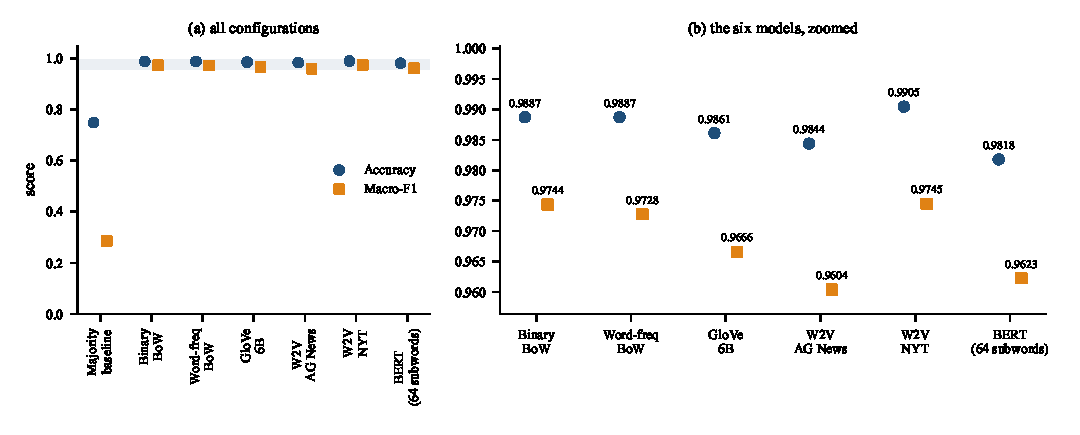
\includegraphics[width=\textwidth]{figs/scores.pdf}
  \caption{各配置的准确率与宏平均 F1。(a) 七种配置放在同一根 0--1 的轴上，
  阴影带标出六个模型占据的区间：它们在轴的顶端挤成一条窄带，而平凡基线远在
  下方。(b) 去掉基线、放宽纵轴以容纳六个模型的全部取值（0.96 到 1.00），它们
  之间的次序这才看得出来——圆点是准确率，方点是宏平均 F1。
  单张图做不到这两件事：0--1 的范围下六个模型不可区分，缩放到窄带后基线会
  落到轴外。}
  \label{fig:scores}
\end{figure*}

\begin{figure*}[t]
  \centering
  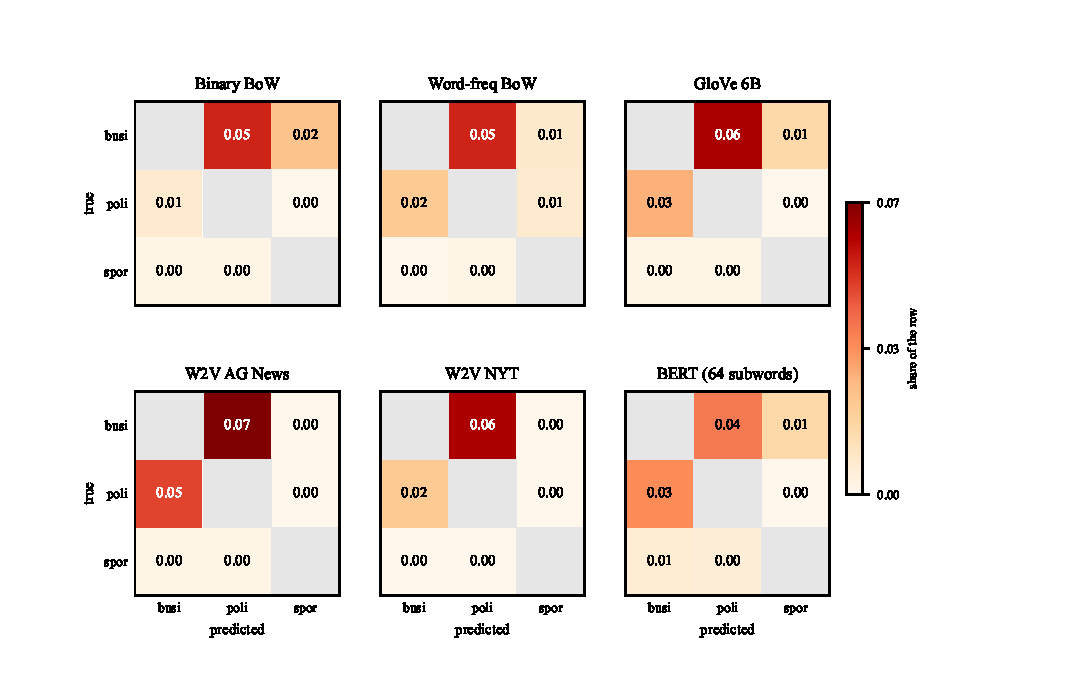
\includegraphics[width=\textwidth]{figs/confusions.pdf}
  \caption{测试集上的行归一化混淆矩阵，\emph{对角线已屏蔽}，色标只覆盖非对角线
  的取值。这样做的原因很实际：对角线在 0.93 以上，与最浅的非对角格子相差一个
  量级，若把两者放进同一根 0--1 的色标，六个面板会全部呈现为一模一样的深色
  对角线，而真正承载论证的那些格子都不到 0.10，完全看不见。屏蔽对角线后，财经
  与政治之间的误判在每一栏都是最深的格子，64 子词的 BERT 那一栏还能看到真实为
  体育的误判（0.01）。逐配置的篇数见表 \ref{tab:errors}。}
  \label{fig:confusions}
\end{figure*}

\begin{table}[t]
\centering
\footnotesize
\caption{测试集上误差的归属（单位：篇），\emph{按真实类别分组}：三列分别是真实为财经、政治、体育的文档中被误判到其他类的篇数，一格一个数。图 \ref{fig:confusions} 按行归一化展示，比例会被类别规模掩盖，这里换算成篇数。}
\label{tab:errors}
\begin{tabular}{lrrr}
\toprule
配置 & 财经 & 政治 & 体育 \\
\midrule
BERT（64 子词） & 7 & 5 & 9 \\
二值词袋 & 10 & 1 & 2 \\
W2V（AG） & 9 & 7 & 2 \\
\bottomrule
\end{tabular}
\end{table}


\section{结果与预测的对比}\label{sec:comparison}

这一节把第 \ref{sec:predictions} 节的五条预测与第 \ref{sec:experiments} 节的
结果逐条对上。三条成立，两条被推翻——被推翻的正是事前写得最具体的那两条，
这大概也是先写预测的价值所在。

本节与下一节会反复引用带随机性配置的多种子区间，这些数字见表
\ref{tab:repeats}；表中的「种子1」即主结果表 \ref{tab:results} 所用的
seed 42，后两列是另跑的种子。

\begin{table}[t]
\centering
\footnotesize
\caption{带随机性配置的重复运行，每格是一个种子的宏平均 F1。词袋与 GloVe 没有随机性，表中未列，其数值是定值。}
\label{tab:repeats}
\begin{tabular}{lrrr}
\toprule
配置 & 种子1 & 种子2 & 种子3 \\
\midrule
W2V（NYT） & 0.9745 & 0.9755 & 0.9710 \\
W2V（AG News） & 0.9604 & 0.9616 & 0.9615 \\
BERT，64 词 & 0.9623 & 0.9538 & 0.9602 \\
BERT，512 词 & 0.9823 & 0.9787 & 0.9800 \\
\bottomrule
\end{tabular}
\end{table}


\subsection{成立的三条}

\paragraph{预测一成立。} 六组配置全部满足宏平均 F1 低于准确率，差距从
\resultGapMin{} 到 \resultGapMax{} 不等。差距最大的是 \resultGapMaxName{}，
它的准确率与宏平均 F1 相差 \resultGapMax{}。这符合预期：多数类占了
四分之三，模型只要把多数类做对，准确率就会很高，而少数类的错误被准确率
平均掉了，却会在宏平均 F1 上完整暴露。

\paragraph{预测二成立，但量级可以忽略。} 二值词袋在测试集上得到
\resultBowFOne{}，词频词袋得到 \resultBowFOneFreq{}，差距 \resultBowPairDiff{}。

这里需要交代一处不完全干净的地方，否则这个差值会被高估。两者的正则强度
$C$ 是在验证集上各自选出来的，而\emph{验证集给出的排序与测试集相反}：验证集上
词频词袋是 \resultBowValFreq{}，高于二值词袋的 \resultBowValBin{}，因此词频
选了更大的 $C$。测试集上两者却调换了次序，而差距只有
\resultBowPairDiff{}。换言之，这个差值建立在一个与测试集判断不一致的
验证集选择之上。第 \ref{sec:setup} 节说词袋管线没有随机性，指的是给定这套
设定后结果可精确复现，不是指两条表示之间的比较不受超参选择影响。

结论因此要弱读：在未归一化的词频表示下，词频这一项没有带来可分辨的额外
信息，二值与词频在本任务上应视为等价。

\paragraph{预测四成立：两者处于同一水平。} 词袋没有随机性，它的 \resultBowFOne{}
是一个定值；NYT 训练的 Word2Vec 三个种子落在 \resultNytVecWorst{} 到
\resultNytVecBest{}，词袋正好落在这个区间之内。同一随机种子下两者的差距是
\resultNytOverBowSameSeed{}。因为一侧是定值、另一侧有波动，这里不适合比较
``两者各自的最好值''，那样会把波动算成表示之间的差异。可以下的判断是：词向量
平均没有拉开优势，严格讲也不是``词袋反超''。这里要留意，这一条只在宏平均 F1 上
成立：按准确率，NYT 词向量的 \resultNytVecAcc{} 反而略高于词袋的 \resultBowAcc{}。
一种解释是词袋用 $|V|$ 个独立坐标轴直接对应关键词的机制，与词向量平均把关键词
稀释在低通滤波里的机制在这个任务上相互抵消——这只是解释，我们没有做能把两种
机制分开的实验。

\subsection{被推翻的两条}

\paragraph{预测三被推翻：前两名调换了位置。} 我们预测 GloVe 依靠数据规模胜出。
实际结果是 NYT 训练的 Word2Vec 最好，GloVe 居中，AG News 训练的 Word2Vec
最差。三个种子下 NYT 训练的取值落在 \resultNytVecWorst{} 到
\resultNytVecBest{}，AG News 训练的落在 \resultAgVecWorst{} 到
\resultAgVecBest{}，GloVe 是没有随机性的定值 \resultGloveScore{}。GloVe
恰好落在另外两者的区间之间，与两边都不重叠。也就是说，预训练词向量被两个
自训练词向量夹在中间，我们预测的第一名掉到了第二名。这个结果说明在这一档数据规模上，
领域契合至少没有输给数据规模。需要立刻补上一句限定：胜出的余量并不大，
第 \ref{sec:profiling} 节会说明这个结论能推到哪里为止。

\paragraph{预测五被推翻，而且是两处同时失效。} 我们预测 BERT 断层式领先，
同时预测 64 个词的截断损失有限。实际上 BERT 以 \resultBertFOne{} 的宏平均 F1
排在末两位，比最好的经典方法低 \resultBertGapToBestAbs{}。而把截断长度从
64 提到 512、其余设置一律不变，宏平均 F1 从 \resultBertFOne{} 升到
\resultBertLenFOne{}，提高了 \resultBertTruncFOneDeltaUns{}，BERT 随即超过
\resultBestNonBert{} 升到第一。所以两条子预测都错了：领先没有出现，
截断的损失也远不是``微弱''。

\section{预测与结果不一致的剖析}\label{sec:profiling}

上一节核对出的两个矛盾各有其成因，本节逐个定位到推理链上出问题的那一环。
先看预测三——它的失效发生在推理的输入端。

\subsection{``数据规模压制领域偏差''为什么没有生效}

预测三的前提是：NYT 训练集太小，Word2Vec 学不准判别性强的词，所以宁可用大规模
通用语料训出来的词向量，哪怕带一点领域偏差。这个前提有两半，逐半检查。

\paragraph{第一半：平均池化只用得上高频词。} 文档向量是词向量的算术平均，出现
一两次的生僻词对结果的贡献被 $1/n$ 稀释掉，决定文档方向的是反复出现的高频词。
而判别三个类别的词恰恰高频：表 \ref{tab:keyword-freq} 列出每类中权重最高的四个
词及其频率，出现最少的一个也有 \resultMinKeywordFreq{} 次，是 \code{min\_count=5}
门槛的约 \resultMinKeywordMultiple{} 倍。

齐夫长尾造成的欠拟合落在低频词上，而低频词在这个池化方式下本来就不起作用。预测
所依赖的失效机制在本任务上没有多少作用面。这证明的是判别词高频，不是``若它们低频
会怎样''——两者不是一回事。

\begin{table}[t]
\centering
\footnotesize
\caption{每个类别中跳过少量通用词后权重最高的四个词，及其在 9{,}215 篇训练文档中的\emph{出现次数}与\emph{出现文档数}，末行给出各自的门槛（前者是 Task 2 的 \code{min\_count}，后者是附录的 \code{min\_df}）。词序是模型的权重序，不是频次序。}
\label{tab:keyword-freq}
\begin{tabular}{llrr}
\toprule
类别 & 词 & 次数 & 篇数 \\
\midrule
体育 & \emph{players} & 7,577 & 3,202 \\
 & \emph{league} & 7,284 & 3,021 \\
 & \emph{season} & 11,719 & 4,494 \\
 & \emph{game} & 17,234 & 5,013 \\
\midrule
政治 & \emph{washington} & 2,937 & 1,743 \\
 & \emph{republican} & 1,466 & 503 \\
 & \emph{obama} & 2,225 & 649 \\
 & \emph{law} & 1,844 & 801 \\
\midrule
财经 & \emph{company} & 2,541 & 924 \\
 & \emph{companies} & 1,409 & 598 \\
 & \emph{market} & 1,558 & 752 \\
 & \emph{chief} & 1,341 & 945 \\
\midrule
门槛 & -- & 5 & 5 \\
\bottomrule
\end{tabular}
\end{table}


\paragraph{第二半：领域偏差被高估。} GloVe 6B 的语料是 2014 年的英文维基百科加
Gigaword\citep{pennington2014glove}，而 Gigaword 本身就是通讯社新闻语料库
\citep{graff2003gigaword}。下游语料谈论的年份也落在相近的时段：提及最多的年份是
\resultYearPeak{}，2010 至 2014 年占 \resultYearTotal{} 次年份提及的
\resultYearShare\%（图 \ref{fig:years}）。

年份提及不等于发稿年份，所以这个统计只界定时间重心的下界。它能支持的结论是：
下游语料谈论的事件落在 GloVe 训练窗口覆盖的年份里，领域偏差更可能来自文体与词表
差异，而非时代错位。

\begin{figure*}[t]
  \centering
  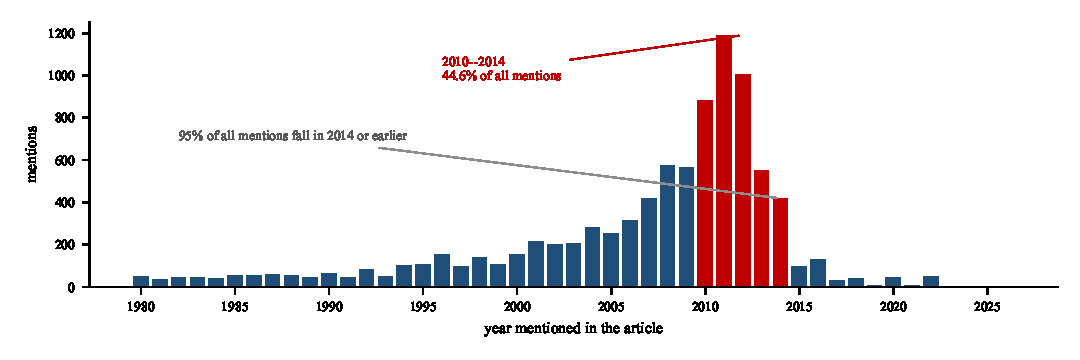
\includegraphics[width=0.86\textwidth]{figs/years.pdf}
  \caption{训练集中提到的年份分布，按年份升序。红色是正文引用的 2010--2014 窗口，
  它占全部 \resultYearTotal{} 次年份提及的 \resultYearShare\%。95\% 的提及落在
  2014 年或更早：这份语料谈论的事件集中在一个 GloVe 6B 训练窗口覆盖的时段里，
  这正是``时代错位''这条解释所能依据的全部内容——它不表明两份语料同属一个时期。}
  \label{fig:years}
\end{figure*}

\paragraph{两点交代。} 覆盖率可以排除一种解释：三种词向量的词元覆盖率分别是
\resultGloveCov{}、\resultNytCov{}、\resultAgCov{}（表 \ref{tab:coverage}），
前两者几乎相同，所以 GloVe 与 NYT 词向量的差距不在``这个词有没有向量''。

GloVe 的预训练语料还可能直接包含测试集原文——若 Gigaword 收录了纽约时报，而这份
下游语料正是纽约时报的稿件。这一点无法核查，也找不到干净的否证办法，只能留在原处。
它的方向偏保守：泄漏只会抬高 GloVe 的成绩，而 GloVe 仍排在 NYT 自训练的词向量
之后。

最后是这条结论的强度。三个种子下 NYT 训练的最差取值比 GloVe 高
\resultNytOverGlove{}，两者区间不重叠；按第 \ref{sec:setup} 节的门槛，这个余量
属于少数几篇文档的差别。可以断言的是``领域内训练不劣于预训练词向量''，不是
``领域内训练稳定胜出''。

\subsection{``倒金字塔救了截断''为什么是错的}

预测五的第二条依赖一个事实主张：倒金字塔结构把主题信息集中在导语，所以前 64
个词已经够用。这是可以直接测量的。

\paragraph{先量截断的代价。} 直接拿 BERT 与词袋比会同时变两件事——表示能力，与
模型看到的词数。要分离后者，先让\emph{同一个}分类器去吃文档的不同前缀：固定用
二值词袋加逻辑回归（Task 1 中最强的配置，且没有随机性），把每篇文档截到前 $N$
个词，扫描 $N$。表示不变，曲线随 $N$ 的变化就只能归因于可见的信息量；这里用
``能读到的词数''作信息量的代理指标。

结果见表 \ref{tab:truncation} 与图 \ref{fig:truncation}。前 64 个词只保留了
\resultTruncShort{} 的宏平均 F1，比读全文低 \resultTruncShortLoss{}；信息量要到
512 个词附近才饱和。

导语确实浓缩了主题，但``浓缩''不等于``完整''：一篇中位长度的报道里，用于分类的
信息有相当一部分落在前 64 个词之外。倒金字塔那条推理把``文章开头最重要''这个
写作学事实，当成了``开头包含足够用于分类的信息''这个信息论结论。

\begin{table}[t]
  \centering
  \footnotesize
  \caption{前缀长度扫描。表示固定为二值词袋加逻辑回归，只有可见的词数变化。
  这就是``读一个前缀要付多少代价''的测量值。}
  \label{tab:truncation}
  \begin{tabular}{rrrr}
\toprule
前缀词数 & 准确率 & 宏平均 F1 & 相对全文 \\
\midrule
16 & 0.9176 & 0.8399 & -0.1345 \\
32 & 0.9410 & 0.8800 & -0.0944 \\
64 & 0.9662 & 0.9288 & -0.0456 \\
128 & 0.9757 & 0.9454 & -0.0290 \\
256 & 0.9861 & 0.9665 & -0.0079 \\
512 & 0.9896 & 0.9750 & +0.0006 \\
全文 & 0.9887 & 0.9744 & -- \\
\bottomrule
\end{tabular}

\end{table}

\paragraph{再量表示能力。} 上面只说明词袋读前缀会损失多少，没有回答``同样的输入
下 BERT 是否更强''。要让它成为直接测量，得让两个模型读到同一段文本，而这里有一个
不能含糊的单位问题：BERT 的 \code{max\_length} 数的是\emph{子词}，词袋那条曲线
截断的是\emph{词}。实测前 64 个子词平均只覆盖 54 个词，前 512 个子词覆盖 408 个
（\code{scripts/prefix\_units.py}），照名义长度直接对比就是两个单位画在同一条轴上。

所以按\emph{每篇文档}各自被 BERT 前缀覆盖到的词数截断词袋，让两个模型读到同一段
文本。结果见表 \ref{tab:matched}：四个匹配点上 BERT 都更高，差值分别是
\resultMatchedGapShort{}、\resultMatchedGapMid{}、\resultMatchedGapLong{}、
\resultMatchedGapFull{}。``表示能力更强''至此才是同一输入下的直接测量。

\begin{table}[t]
\centering
\scriptsize
\caption{真正同输入下的对比。词袋一侧按\emph{每篇文档}实际被 BERT 前缀覆盖到的词数截断，而不是按同一个名义 $N$，因为 $N$ 在两侧分别是词与子词。}
\label{tab:matched}
\begin{tabular}{rrrrr}
\toprule
BERT 前缀（子词） & 覆盖词数 & 词袋 & BERT & 差值 \\
\midrule
64 & 54 & 0.9338 & 0.9623 & +0.0285 \\
128 & 108 & 0.9361 & 0.9773 & +0.0412 \\
256 & 214 & 0.9642 & 0.9787 & +0.0145 \\
512 & 408 & 0.9749 & 0.9823 & +0.0074 \\
\bottomrule
\end{tabular}
\end{table}


\begin{figure*}[t]
  \centering
  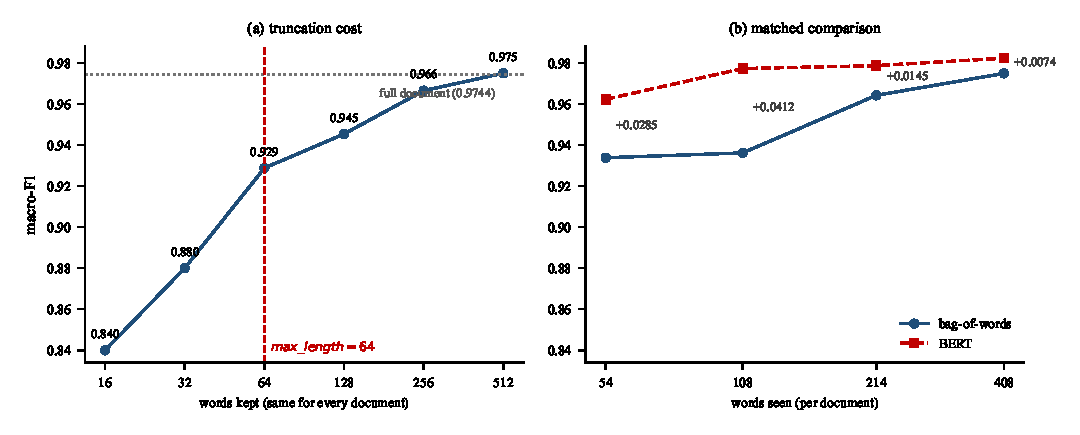
\includegraphics[width=\textwidth]{figs/truncation.pdf}
  \caption{两个不同的问题。(a) 截断代价：表示固定为词袋，\emph{每篇文档}都截到
  同样的 $N$ 个词，曲线说明一篇报道的前 $N$ 个词里有多少可用于分类的信息。
  (b) 匹配比较：词袋按\emph{每篇文档}实际被 BERT 前缀覆盖的词数截断，两个模型
  读同一段文本，标注的是两者的差值。两个面板的\emph{横轴含义不同}（前者是每篇都
  截到同一个 $N$，后者是各篇实际被覆盖的词数），因此没有画在同一面板里；但两者
  画的是同一个量（宏平均 F1），所以\emph{共用一个纵轴范围}，以免并排比较时被
  不同的刻度误导。}
  \label{fig:truncation}
\end{figure*}

两处细节。表 \ref{tab:matched} 与表 \ref{tab:truncation} 的词袋取值不同，
因为前者按每篇各自的覆盖词数截断、后者把每篇都截到同一个 $N$，两套规则不可互推。
另外差值并不随可见词数单调收窄：词袋那一侧换一组截断词数再算（\resultDenseBowWords{}
个词）得到 \resultDenseBowCurve{}，自身就不单调，而 BERT 一侧的四个点单调递增。
这个走势因此无从解释，能支持的只是``每个匹配点上 BERT 都更高，且在最长的两档上
差距明显缩小''。

\subsection{代价落在哪些文档上}

截断的代价不是均匀分布的。表 \ref{tab:by-length} 把测试集按词数分成五层，报告
每层上两个模型的错误率，以及 BERT 的前缀平均能覆盖该层文档的多大比例。

最明显的反差在第一层：200 词以下 BERT 的错误率是 \resultByLenShortBert{}，
词袋是 \resultByLenShortBow{}，因为这一层的前缀就覆盖了 \resultSeenShort{} 的
内容。但这一层只有 76 篇，两个错误率折成篇数是 0 篇对 2 篇，而相邻的 200 至 400
词层反过来是 1 篇对 0 篇——这个量级的差别在噪声之内。真正站得住的是长文档那一端：
700 至 1000 词层有 \resultDocsPeak{} 篇文档，词袋错误率 \resultByLenPeakBow{}，
BERT 是 \resultByLenPeakBert{}。

BERT 的错误率在这里不是单调的：700 至 1000 词层最高，更长的层反而略低。这个形状
不必解释——五层的错误篇数分别是 0、1、1、14、5，总共 21 篇，层间只差几篇。顺便
排除一个候选解释：极长文档并不特别偏向体育，>1000 词层有 \resultLongestBinDocs{}
篇，其中 \resultLongestBinSports{}\% 是体育，与全文的 75\% 相当。

\begin{table}[t]
\centering
\scriptsize
\caption{测试集按文档长度分层。``可见比例''是 BERT 的 64 个子词前缀平均覆盖到的文档比例。两个模型的错误率都以该层文档数为分母。}
\label{tab:by-length}
\begin{tabular}{rrrrr}
\toprule
长度（词） & 篇数 & 可见 & 词袋错 & BERT 错 \\
\midrule
<200 & 76 & 39.7\% & 2.6\% & 0.0\% \\
200--400 & 101 & 17.6\% & 0.0\% & 1.0\% \\
400--700 & 304 & 9.7\% & 0.3\% & 0.3\% \\
700--1000 & 464 & 6.5\% & 1.3\% & 3.0\% \\
>1000 & 208 & 4.9\% & 1.9\% & 2.4\% \\
\midrule
全部 & 1153 & 10.2\% & 1.1\% & 1.8\% \\
\bottomrule
\end{tabular}
\end{table}


\paragraph{一个具体例子。} 原始语料中 \code{idx} 为 5252 的文档是一篇 1{,}166 词的
体育报道（语料行号，不是测试集序号），BERT 判为财经，词袋判对。BERT 只读到前 48
个词：

\begin{quote}\small
edina, minn. --- the 95-degree heat on a late august day made josh harding hasten
from his cadillac escalade pickup truck into an air-conditioned coffee shop. a few
minutes after buying a lemonade, harding --- in a white t-shirt, dark blue shorts,
flip-flops
\end{quote}

这一段里没有任何体育线索。而紧接着的下一个词是
``and a backward minnesota twins ball cap''，随后出现
``the minnesota wild goalie \dots\ during the n.h.l. lockout''。判别这篇报道属于
体育的标志词恰好落在截断点之后。这个例子只解释 BERT \emph{为什么没有看到体育}，
不解释它为什么归到财经。

\paragraph{代价落在哪些文档上，可以做一个差分。} 测试集里``BERT 判错而词袋判对''
的文档共 \resultBertWrongBowRight{} 篇（由两个模型的逐文档预测文件对比得出，
不在上表中）。按长度分布是 0、1、1、11、4 篇，其中
\resultBertWrongBowRightLong{} 篇落在最长的两层，与上面分层表里 BERT 的错误
集中在长文档一致。这组数字是差分对照：同一批文档上 BERT 错而词袋对，所以差异
只能来自截断。

\subsection{约束条件能推多远}

本文比较的是\emph{作业规定的那一组配置}，不是``词袋优于 BERT''。在中位长度
\resultMedianTokens{} 个词元、截断到 64 个子词这两个条件同时成立时，读全文的
词袋会赢；把截断放宽，结论立刻反转。若换一个类别词汇交叠更多的语料，方法之间的
排序是否会更分明，本报告无从判断——手头只有一份带标签的下游语料。

\begin{table}[t]
\centering
\footnotesize
\caption{每个类别权重最高的 50 个词中任意两类的交集大小。这里的词表未剔除任何通用词，唯一的非零交集 \emph{mr.} 正是这一类词；表 \ref{tab:keyword-freq} 用的则是剔除后的词表。对角线是类别与自身，最右列各给两个例词。}
\label{tab:discriminative}
\begin{tabular}{lccc@{\hspace{8pt}}l}
\toprule
类别 & 财经 & 政治 & 体育 & 例词 \\
\midrule
财经 & -- & 1 & 0 & company、companies \\
政治 & 1 & -- & 0 & washington、republican \\
体育 & 0 & 0 & -- & players、league \\
\bottomrule
\end{tabular}
\end{table}


三类的词汇几乎不重叠是这份语料的特点：体育类的 F1 在六种模型配置下都不低于
\resultSportsFOneMin{}。剩余误差的落点则因表示而异。表 \ref{tab:errors} 按真实
类别统计了三个配置：两个经典配置的误差主要来自真实为财经或政治的文档（二值词袋
\resultErrBowBizPol{} 篇对 \resultErrBowSports{} 篇；AG News 词向量
\resultErrAgVecBizPol{} 篇对 \resultErrAgVecSports{} 篇），而 64 子词的 BERT 上
两者已经相当（\resultErrBertBizPol{} 篇对 \resultErrBertSports{} 篇）。

带随机性的配置各跑了三个种子，相邻名次之间小于 0.005 的差距不做强断言。BERT 的
64 子词配置三个种子落在 \resultBertSeedsWorst{} 到 \resultBertSeedsBest{}，而
AG News 词向量落在 \resultAgVecWorst{} 到 \resultAgVecBest{}，两个区间\emph{重叠}。
所以``BERT 排在最后''需要限定：它低于 NYT 词向量（差 \resultNytGapToBert{}）与
二值词袋（差 \resultBowGapToBert{}）是确定的，与 AG News 词向量、GloVe
（差 \resultBertOverGlove{}）则都不足以强断言。

截断长度这一项相反，是可以强断言的。64 子词配置三个种子落在
\resultBertSeedsWorst{} 到 \resultBertSeedsBest{}，512 子词配置落在
\resultBertLenSeedsWorst{} 到 \resultBertLenSeedsBest{}，两个区间
\resultTruncRangesOverlap：拿 512 最差的种子比 64 最好的种子，仍有
\resultTruncMinGain{} 的差距，且 512 的每一个种子都高于全部经典配置。

\section{结论}

第一，在这个任务上，经典词袋表示的能力与最好的稠密词向量平均处在同一水平，
而它不需要任何预训练权重，训练也不依赖 GPU。三个稠密来源中 AG News 训练的
Word2Vec 明显更低，``同一水平''不涵盖它。六种配置全部落在
\resultRangeLow{} 到 \resultRangeHigh{} 之间，跨度 \resultEmbedSpread{}；而同一
模型内最易的类与最难的类之间，F1 相差 \resultClassGap{}（以二值词袋为例）。
比较表示方法带来多大差别，应当参照前者。这个结果
大概来自三类新闻的词汇几乎不重叠，不过这只是一条解释：本报告为``为什么各方法
挤在一起''给过几种机制，它们都与观察相容，我们没有做能把它们区分开的实验。

第二，宏平均 F1 而非准确率才是有效的指标。平凡基线取得 \resultMajorityAcc{}
的准确率，却对两个少数类完全无能为力。

第三，先写预测再做实验，在我们这次是有收益的。事前写得最具体的两条预测都被
推翻了，推翻它们的过程产生了本报告最有信息量的两个结果。两条观察不足以支撑
一条方法学结论，只能算一次经验。

第四，不要把配置限制的后果归于方法本身。BERT 在这份报告里排在末两位，原因不是
上下文表示不好，而是它只被允许读文档的十分之一。把截断放宽到 512 个子词，它在
每一个种子下都成为最好的配置。任何来自受限配置的实验数字，都是关于那个配置的
陈述。

第五，测量要针对机制而不是针对现象。预测五出错的地方，是它用一个写作学观察
（导语最重要）替代了一个信息论判断（导语包含足够信息）。补上这一步测量的做法是
让同一个分类器去读不同长度的前缀，把信息量这一个变量单独分离出来。

\section{复现说明}

代码仓库包含完整流程。在项目根目录下依次执行：

\begin{itemize}[leftmargin=1.4em,itemsep=1pt]
  \item \code{uv sync}，安装锁定版本的运行环境。
  \item \code{uv run python -m scripts.make\_splits}，生成共用的 80/10/10 划分。
  \item \code{uv run python -m scripts.task1\_bow}，Task 1。
  \item \code{uv run python -m scripts.task2\_embed --variant \{glove,
        w2v\_ag, w2v\_nyt\}}，Task 2。
  \item \code{uv run python -m scripts.task3\_bert}，Task 3。
  \item \code{uv run python -m scripts.truncation\_curve}，第 \ref{sec:profiling}
        节的截断代价扫描（表 \ref{tab:truncation}）。
  \item \code{uv run python -m scripts.prefix\_units} 与
        \code{uv run python -m scripts.matched\_prefix}，同一节里子词到词的换算
        与匹配比较（表 \ref{tab:matched}）。
  \item \code{uv run python -m scripts.topic\_diagnostics}，第 \ref{sec:setup}
        与 \ref{sec:profiling} 节用到的判别词、词频与年份统计。
  \item \code{uv run python -m scripts.error\_analysis}，表 \ref{tab:by-length}
        的分层错误率与第 \ref{sec:profiling} 节的具体误判样例。
  \item \code{uv run python -m scripts.collect\_results} 与
        \code{uv run python -m scripts.make\_figs}，从 \code{results/} 重新生成
        本报告的全部表格与插图。
  \item \code{./scripts/build\_report.sh}，重新生成并编译本文档。
\end{itemize}

重复运行使用 \code{--seed} 参数，例如
\code{--seed 7 --suffix \_seed7}。附录实验使用 \code{--min-df 5} 与
\code{--max-len 512}。

\appendix
\section{附录}\label{sec:appendix}

这一节包含一组辅助实验：检验 Task 1 的词表剪枝是否影响结论。（把 BERT 的
截断长度放宽到 512 的那组对照，因为与正文第 \ref{sec:profiling} 节论证直接
相关，已放在附录表 \ref{tab:appendix} 的最后一行，正文中随用随引。）

\subsection{词表剪枝是否是承重设计}

主实验使用 \code{min\_df=1}，即作业``整个训练语料的词表''的字面实现，得到
\resultVocabSize{} 个词。这么大的词表以只出现一次的词为主，因此我们的结论
是否依赖它们需要检验。把 \code{min\_df} 改为 5 之后词表剩下原来的 \resultVocabShrink{}，宏平均 F1 的变化不超过 \resultMinDfMaxDelta{}，见表 \ref{tab:appendix}。词表剪枝
不承重：区分这三个类别的信息集中在常见词里，这与表 \ref{tab:discriminative}
测出的判别词集一致。需要留意这里用的是哪个量：\code{min\_df} 按\emph{文档频率}
剪枝，所以支持``它们不会被剪掉''的是出现文档数而非出现次数（第
\ref{sec:experiments} 节专门区分过这两个量）。表 \ref{tab:keyword-freq} 给出的是``出现次数/出现文档数''，后者的最小值是 \resultMinKeywordDocFreq{} 篇，
因此 \code{min\_df} 取到约 500 都不会剪掉这些词；我们没有试过更激进的剪枝。

附带一点：在 \code{min\_df=1} 下词频词袋略逊于二值词袋，在 \code{min\_df=5}
下反了过来。这个方向反转与第 \ref{sec:comparison} 节说的验证集、测试集
排序不一致是同一件事：两者的差距本身就落在超参选择的量级内，换个词表
阈值就足以改变次序。这也再次说明这两个表示没有实质差别。

\begin{table*}[h]
\centering
\footnotesize
\caption{附录实验。前两行把 Task 1 的 \texttt{min\_df} 改为 5；最后一行把 BERT 的截断长度改为 512，用于把表示能力与截断的代价分开。}
\label{tab:appendix}
\begin{tabular}{lrrr}
\toprule
配置 & $\lvert V \rvert$ & 准确率 & 宏平均 F1 \\
\midrule
二值词袋，min\_df=5 & 28,938 & 0.9887 & 0.9744 \\
词频词袋，min\_df=5 & 28,938 & 0.9887 & 0.9745 \\
BERT，max\_len 512 & -- & 0.9931 & 0.9823 \\
\bottomrule
\end{tabular}
\end{table*}


\bibliography{references}

\end{document}
